% Encoding: UTF-8
%%%%%%%%%%%%%%%%%%%%%%%%%%%%%%%%%%%%%%%%%%%%%%%%%%%%%%%%%%%%%%%%%%%%%%%%%%%%%%%

%%%%%%%%%%%%%%%%%%%%%%%%%%%%%%%%%%%%%%%%%%%%%%%%%%%%%%%%%%%%%%%%%%%%%%%%%%%%%%%
% $Id: slides.tex 17 2011-02-10 15:21:56Z klugeflo $
%%%%%%%%%%%%%%%%%%%%%%%%%%%%%%%%%%%%%%%%%%%%%%%%%%%%%%%%%%%%%%%%%%%%%%%%%%%%%%%

%%%%%%%%%%%%%%%%%%%%%%%%%%%%%%%%%%%%%%%%%%%%%%%%%%%%%%%%%%%%%%%%%%%%%%%%%%%%%%%
%%
%% Vorlage fuer LaTeX-Beamer
%% gemaess dem Corporate Design der Uni Augsburg
%%
%%%%%%%%%%%%%%%%%%%%%%%%%%%%%%%%%%%%%%%%%%%%%%%%%%%%%%%%%%%%%%%%%%%%%%%%%%%%%%%
%%
%% Changelog:
%%
%% 11/02/10 (FAK) Start
%%
%%%%%%%%%%%%%%%%%%%%%%%%%%%%%%%%%%%%%%%%%%%%%%%%%%%%%%%%%%%%%%%%%%%%%%%%%%%%%%%


%%%%%%%%%%%%%%%%%%%%%%%%%%%%%%%%%%%%%%%%%%%%%%%%%%%%%%%%%%%%%%%%%%%%%%%%%%%%%%%

\documentclass[xcolor=pdftex,dvipsnames,table]{beamer}

%%%%%%%%%%%%%%%%%%%%%%%%%%%%%%%%%%%%%%%%%%%%%%%%%%%%%%%%%%%%%%%%%%%%%%%%%%%%%%%

% Language settings
% IMPORTANT: If you change the language settings, make sure to run
% cleantex prior to any latex/pdflatex to remove all .aux files, else
% latex might fail!
\usepackage[english]{babel}
%\usepackage[german]{babel}

%\usepackage{graphicx}
\usepackage[utf8]{inputenc}
%\usepackage{mathptmx}


%%%%%%%%%%%%%%%%%%%%%%%%%%%%%%%%%%%%%%%%%%%%%%%%%%%%%%%%%%%%%%%%%%%%%%%%%%%%%%%

\usetheme{fai}

% IMPORTANT/TODO: currently only PDF graphic files should be used, PNG
% or JPEG may harm the Adobe Reader colour palette and result in
% strange display colours.
%\DeclareGraphicsExtensions{.pdf}

\graphicspath{{./img/}}

%%%%%%%%%%%%%%%%%%%%%%%%%%%%%%%%%%%%%%%%%%%%%%%%%%%%%%%%%%%%%%%%%%%%%%%%%%%%%%%
%% Presentation main settings
%%%%%%%%%%%%%%%%%%%%%%%%%%%%%%%%%%%%%%%%%%%%%%%%%%%%%%%%%%%%%%%%%%%%%%%%%%%%%%%

\title[Organic Computing 2]{Lösungsvorschlag Blatt06}
\subtitle{Spieleprogrammierung}
\author{Victor Gerling, Qiang Chang, Lukas Huhn}
\institute[Uni Augsburg]{Institut für Informatik, Lehrstuhl für Organic Computing}
\date[]{\\\today}


%%%%%%%%%%%%%%%%%%%%%%%%%%%%%%%%%%%%%%%%%%%%%%%%%%%%%%%%%%%%%%%%%%%%%%%%%%%%%%%
%% Main Document starts here
%%%%%%%%%%%%%%%%%%%%%%%%%%%%%%%%%%%%%%%%%%%%%%%%%%%%%%%%%%%%%%%%%%%%%%%%%%%%%%%

\begin{document}

\begin{frame}
  \titlepage
\end{frame}

\section*{Aufgabe 1}
\begin{frame}
  \frametitle{Aufgabe 1}
  \begin{itemize}
  		\item Ansteuerung der BlackBox
  	  \item \url{https://git.rz.uni-augsburg.de/bosserda/oc/blob/master/src/Optimierung/DockerAdapter.java}
  \end{itemize}
\end{frame}

%%%%%%%%%%%%%%%%%%%%%%%%%%%%%%%%%%%%%%%%%%%%%%%%%%%%%%%%%%%%%%%%%%%%%%%%%%%%%%%

\section*{Aufgabe 2, 3}
\begin{frame}
  \frametitle{Aufgabe 2, 3}
  \begin{itemize}
  		\item HillClimbing
  	  	\item \url{https://git.rz.uni-augsburg.de/bosserda/oc/blob/master/src/Optimierung/HillClimbing.java}
  	  	\item Simulated Annealing
  	  	\item \url{https://git.rz.uni-augsburg.de/bosserda/oc/blob/master/src/Optimierung/SimulatedAnnealing.java}
  \end{itemize}
\end{frame}

%%%%%%%%%%%%%%%%%%%%%%%%%%%%%%%%%%%%%%%%%%%%%%%%%%%%%%%%%%%%%%%%%%%%%%%%%%%%%%%

\section*{Aufgabe 4}

\begin{frame}
  \frametitle{Aufgabe 4.1}
  \begin{itemize}
  		\item Lassen Sie die oben verlangten Parametrisierungen der Verfahren (insgesamt 8-mal Hill-Climbing
und 4-mal Simulated Annealing) 10-mal für jede der Blackboxen für 500 Iterationen laufen. Betrachten
Sie für jede der Blackboxen ausschließlich den Wertebereich $[-1000; 1000]$.
  \end{itemize}
\end{frame}

\begin{frame}
  \frametitle{Aufgabe 4.2}
  \begin{itemize}
  		\item Erstellen Sie für jede Blackbox für die Hill-Climbing-Durchgänge ein Iteration-Optimumsfitness-
Diagramm in das Sie den durchschnittlichen (über die 10 Versuche) Verlauf des Fitnesswerts des
bisher bekannten besten Werts einzeichnen.
  \end{itemize}
\end{frame}

\begin{frame}
  \frametitle{Aufgabe 4.3}
  \begin{itemize}
  		\item Erstellen Sie ein Iteration-Temperatur-Diagramm für die Abkühlungsfunktionen mit den von
Ihnen gewählten Parametern.
\newline
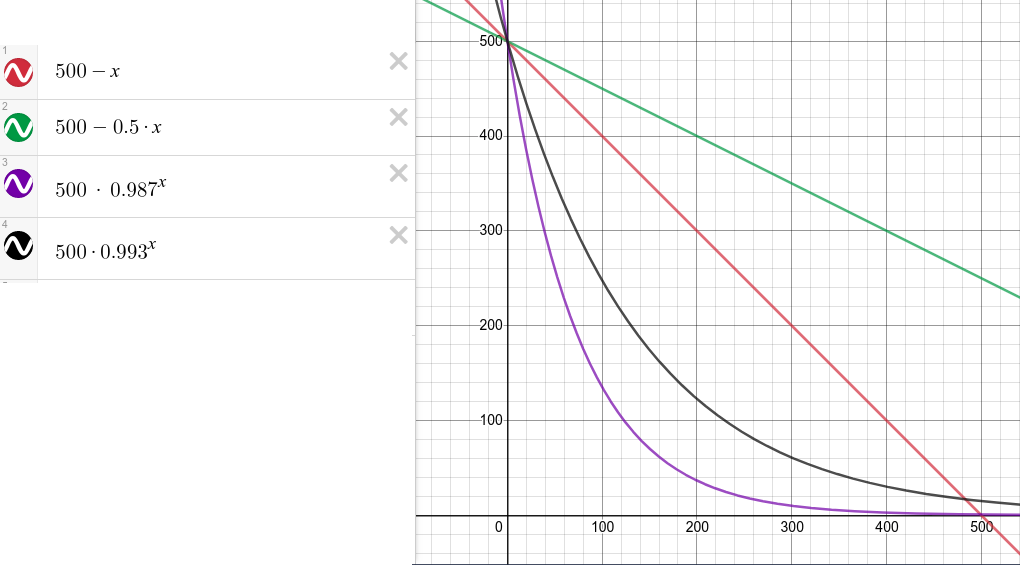
\includegraphics[scale=0.3]{img/OC2_Blatt6_A4_3.png}
  \end{itemize}
\end{frame}


\begin{frame}
  \frametitle{Aufgabe 4.4}
  \begin{itemize}
  		\item Erstellen Sie für jede Blackbox für die Simulated-Annealing-Durchgänge ein Iteration-Optimumsfitness-
Diagramm in das Sie den durchschnittlichen (über die 10 Versuche) Verlauf des Fitnesswerts
des bisher bekannten besten Werts jeder Blackbox einzeichnen.
  \end{itemize}
\end{frame}

\begin{frame}
  \frametitle{Aufgabe 4.4}
  \begin{itemize}
  		\item Erstellen Sie für jede Blackbox für die Simulated-Annealing-Durchgänge ein Iteration-Optimumsfitness-
Diagramm in das Sie den durchschnittlichen (über die 10 Versuche) Verlauf des Fitnesswerts
des bisher bekannten besten Werts jeder Blackbox einzeichnen.
  \end{itemize}
\end{frame}

\begin{frame}
  \frametitle{Aufgabe 4.5}
  \begin{itemize}
  		\item Erstellen Sie ein Iteration-Optimumsfitness-Diagramm (wie vorher), in das Sie die besten beiden
Hill-Climbing-Parametrisierungen, die besten beiden Simulated-Annealing-Parametrisierungen sowie
das einfache Verfahren vom vorherigen Übungsblatt einzeichnen.
  \end{itemize}
\end{frame}

\begin{frame}
  \frametitle{Aufgabe 4.6}
  \begin{itemize}
  		\item Geben Sie eine Tabelle der durch die verschieden parametrisierten Verfahren (inklusive des
Verfahrens vom vorherigen Blatt) erreichten Optima und deren jeweiligen Fitnesswert an und
markieren Sie für jede Blackbox den besten Fitnesswert.
  \end{itemize}
\end{frame}

\begin{frame}
  \frametitle{Aufgabe 4.7}
  \begin{itemize}
  		\item Welche der Verfahren konnten bei 500 Schritten bei welchen der Blackboxen (vermutlich) konvergieren?
Woran machen Sie das fest?
  \end{itemize}
\end{frame}


\end{document}

%%%%%%%%%%%%%%%%%%%%%%%%%%%%%%%%%%%%%%%%%%%%%%%%%%%%%%%%%%%%%%%%%%%%%%%%%%%%%%%
